\documentclass{beamer}

\usepackage{wasysym}
\usepackage[center]{caption}

% === ENCODINGS === 

\usepackage[english, russian]{babel}
\usepackage[T2A]{fontenc}
\usepackage[utf8]{inputenc}

% === MATH === 

% Some math fonts
\usepackage{amsfonts}

% Some math symbols
\usepackage{amssymb}

% Some math "making beautiful" stuff
\usepackage{mathtools}

% Some math fonts
\usepackage{mathrsfs}  

\numberwithin{equation}{section}

% === REFERENCES ===

\usepackage[sorting=none]{biblatex}
\addbibresource{sources.bib}


% === MY COMMANDS ===

\newcommand{\deriv}[2]{\frac{\partial #1}{\partial #2}}
\newcommand{\R}{\mathbb R}
\newcommand{\Row}{\sum\limits_{n=1}^\infty}
\newcommand{\Rowk}{\sum\limits_{k=1}^\infty}
\newcommand{\Prod}{\prod\limits_{n=1}^\infty}
\newcommand{\Prodk}{\prod\limits_{k=1}^\infty}
\newcommand{\eps}{\varepsilon}
\renewcommand{\phi}{\varphi}
\newcommand{\fall}{\:\forall\:}
\newcommand{\ex}{\:\exists\:}

% === MATH OPERATORS ===

\DeclareMathOperator{\const}{const}
\DeclareMathOperator{\Ker}{ker}
\DeclareMathOperator{\Image}{im}
\DeclareMathOperator{\Def}{def}
\DeclareMathOperator{\Rank}{rank}
\DeclareMathOperator{\Dim}{dim}
\DeclareMathOperator{\Argmin}{Argmin}
\DeclareMathOperator{\Tr}{tr}
\DeclareMathOperator{\Interior}{int}
\DeclareMathOperator{\Dom}{dom}
\DeclareMathOperator{\Aff}{aff}
\DeclareMathOperator{\Relint}{relint}

% === OTHER ===

% Indent in the begging of first par
\usepackage{indentfirst}



\title[OST. Фонтанные коды]{Использование идей фонтанного кодирования 
при передаче малого числа битовых пакетов}
\author[Иванов Е.Р.]{Иванов Егор Романович, 317 группа \\ 
Научный руководитель: к.ф.-м.н. Гуров Сергей Исаевич}
\date{\today}
\institute{ММП ВМК МГУ}

\titlegraphic{
\includegraphics[scale=0.12]{img/msu.eps}}
\usetheme{Madrid}

\begin{document}

\begin{frame}{One-slide Talk}

    \begin{tabular}{cl}  
         \begin{tabular}{c}
           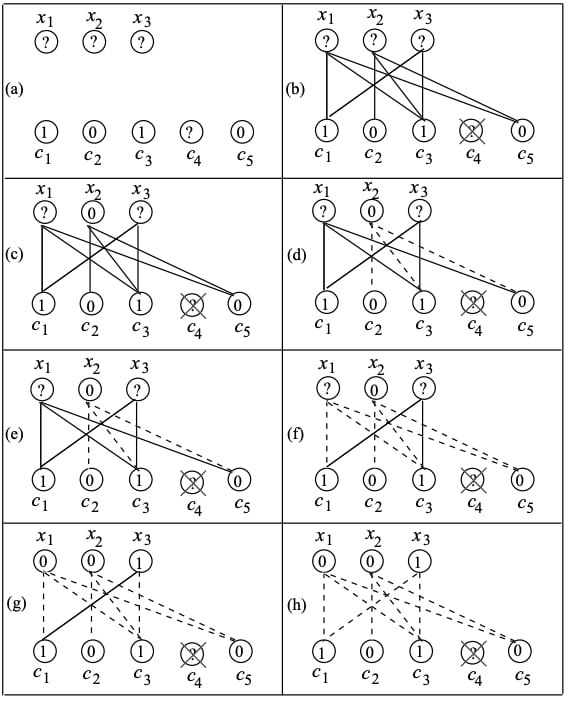
\includegraphics[width=0.35\linewidth]{img/lt_process.jpg}
           \end{tabular}
           & \begin{tabular}{l}
             \parbox{0.53\linewidth}{%  change the parbox width as appropiate
             Задача передачи битовых пакетов по каналу связи:
             \begin{itemize}
                 \item код \textit{систематический}
                 \item модель канала -- \textit{<<очень хороший>>} BEC
                 \item при одних и тех же параметрах высылается \textit{малое} число пакетов
             \end{itemize}
             \textbf{Требуется:} используя идеи фонтанного кодирования, сделать канал \textit{идеальным}.
             }
    \end{tabular}  \\
    \end{tabular}

\end{frame}

\end{document}
